\documentclass[UTF8,a4paper,11pt]{ctexart}

\usepackage{geometry}
\usepackage{amsmath,amssymb}
\usepackage{booktabs}
\usepackage{graphicx}
\usepackage{float}
\usepackage{hyperref}
\usepackage{enumitem}

\geometry{left=2.5cm,right=2.5cm,top=2.5cm,bottom=2.5cm}
\graphicspath{{figures/}}
\hypersetup{colorlinks=true,linkcolor=blue,citecolor=blue,urlcolor=blue}

\title{基于稀疏测量的 CSI 空间外推\\
\large 多场景数据集、复数线性插值与物理引导 Fourier MLP}
\author{姓名：\underline{\hspace{4cm}}\qquad 学号：\underline{\hspace{4cm}}}
\date{\today}

\begin{document}

\maketitle

\begin{abstract}
本文面向研究探索任务 D，首先构建一个可复现的小规模合成空间 CSI 数据集，为后续稀疏测量外推实验提供统一真值。
数据集包含 10 个传播场景、8 个子载波以及每场景 $101\times101$ 个空间位置；每个场景由一条直达径和三条反射径组成，并随机改变发射机位置、反射点、复数反射系数和路径损耗指数。
最终 CSI 以复数形式保存，数据张量形状为 $10\times8\times101\times101$。
本文同时进行数值完整性、场景差异、子载波差异和空间 Nyquist 条件检查。
在数据集验证完成后，本文进一步在独立测试场景上运行复数线性插值 baseline，比较 $5\%$、$10\%$ 和 $20\%$ 随机空间测量。结果表明，在当前快速相位变化条件下，增加采样率并未自动降低复数 NMSE、幅度 NMAE 和相位 MAE，说明普通线性插值不适合直接恢复高频复数 CSI。
随后实现 Fourier-feature MLP 作为改进方法。该模型的 NMSE 接近 $0\,\mathrm{dB}$，但幅度 NMAE 约为 $0.90$、相位 MAE 接近随机相位参考值，重建图显示其退化为接近零预测。该失败实验说明，较低的单一 NMSE 不等于有效 CSI 恢复，必须联合检查幅度、相位与可视化结果。
基于失败原因，本文进一步利用已知 Tx 位置和子载波频率补偿直达径相位，再用相同 Fourier MLP 学习补偿后的复数场。在 $5\%$、$10\%$ 和 $20\%$ 测量下，该方法分别取得 $-13.29$、$-14.85$ 和 $-15.84\,\mathrm{dB}$ 的复数 NMSE，并显著降低幅度和相位误差，验证了传播物理先验对稀疏 CSI 外推的重要性。
\end{abstract}

\section{任务目标}

设场景编号为 $s$，空间位置为 $\mathbf p=(x,y)$，子载波频率为 $f_k$，完整复数 CSI 为
\begin{equation}
    H_s(\mathbf p,f_k)\in\mathbb C.
\end{equation}
任务最终需要只提供 $5\%$、$10\%$ 或 $20\%$ 空间位置的 CSI，恢复其余未知位置，并比较简单 baseline 与一种改进方法。

本阶段的目标不是训练预测模型，而是先得到满足以下条件的统一数据集：
\begin{enumerate}[label=(\arabic*)]
    \item 包含多个不同传播场景；
    \item 包含多条传播路径；
    \item 每个空间位置包含多个子载波的复数 CSI；
    \item 训练、验证和测试场景相互独立；
    \item 空间网格足以表示 $3\,\mathrm{GHz}$ 附近的快速相位变化。
\end{enumerate}

\section{数据生成模型}

\subsection{空间网格与子载波}

空间区域大小为 $4\,\mathrm m\times4\,\mathrm m$，使用 $101\times101$ 规则网格，相邻位置间距为
\begin{equation}
    \Delta x=\Delta y=\frac{4}{101-1}=0.04\,\mathrm m.
\end{equation}

数据集包含 8 个等间隔子载波，中心频率为 $3\,\mathrm{GHz}$，总带宽为 $20\,\mathrm{MHz}$：
\begin{equation}
    f_k\in[2.99,3.01]~\mathrm{GHz},\qquad k=0,\ldots,7.
\end{equation}

\subsection{直达路径}

场景 $s$ 中发射机位置为 $\mathbf p_{\mathrm{Tx},s}$，接收位置为 $\mathbf p$，直达距离为
\begin{equation}
    d_{s,0}(\mathbf p)=
    \|\mathbf p-\mathbf p_{\mathrm{Tx},s}\|_2.
\end{equation}
直达 CSI 为
\begin{equation}
    H_{s,0}(\mathbf p,f_k)=
    \frac{1}{(d_{s,0}(\mathbf p)+\epsilon)^{\eta_s/2}}
    \exp\left(-j\frac{2\pi f_k d_{s,0}(\mathbf p)}{c}\right).
\end{equation}

\subsection{反射路径}

每个场景包含三个反射点 $\mathbf q_{s,l}$。第 $l$ 条反射路径长度为
\begin{equation}
    d_{s,l}(\mathbf p)=
    \|\mathbf p_{\mathrm{Tx},s}-\mathbf q_{s,l}\|_2
    +\|\mathbf q_{s,l}-\mathbf p\|_2.
\end{equation}
对应反射分量为
\begin{equation}
    H_{s,l}(\mathbf p,f_k)=
    \frac{\rho_{s,l}}{(d_{s,l}(\mathbf p)+\epsilon)^{\eta_s/2}}
    \exp\left(-j\frac{2\pi f_k d_{s,l}(\mathbf p)}{c}\right),
\end{equation}
其中 $\rho_{s,l}$ 是包含幅度衰减和额外相位偏移的复数反射系数。

总 CSI 为复数相干叠加：
\begin{equation}
    H_s(\mathbf p,f_k)=
    H_{s,0}(\mathbf p,f_k)
    +\sum_{l=1}^{3}H_{s,l}(\mathbf p,f_k).
\end{equation}

\section{数据集配置}

\begin{table}[H]
    \centering
    \caption{初始 CSI 数据集配置}
    \label{tab:dataset-config}
    \begin{tabular}{ll}
        \toprule
        项目 & 设置 \\
        \midrule
        随机种子 & 2026 \\
        场景数量 & 10 \\
        每场景反射路径数量 & 3 \\
        子载波数量 & 8 \\
        空间区域 & $4\,\mathrm m\times4\,\mathrm m$ \\
        网格大小 & $101\times101$ \\
        网格间距 & $0.04\,\mathrm m$ \\
        中心频率 & $3\,\mathrm{GHz}$ \\
        总带宽 & $20\,\mathrm{MHz}$ \\
        路径损耗指数范围 & $[2.6,3.4]$ \\
        反射系数幅度范围 & $[0.25,0.65]$ \\
        CSI 数据类型 & \texttt{complex64} \\
        CSI 张量形状 & $(10,8,101,101)$ \\
        \bottomrule
    \end{tabular}
\end{table}

每个场景随机生成发射机位置、三个满足最小间距约束的反射点、复数反射系数和路径损耗指数。
场景按照 $6:2:2$ 划分为训练、验证和测试集合：
\begin{align}
    \mathcal S_{\mathrm{train}} &= \{0,2,3,4,5,9\},\\
    \mathcal S_{\mathrm{val}} &= \{1,7\},\\
    \mathcal S_{\mathrm{test}} &= \{6,8\}.
\end{align}

\section{数据完整性验证}

生成脚本保存数据后会重新读取文件，再执行自动检查。结果见表~\ref{tab:validation}。

\begin{table}[H]
    \centering
    \caption{数据集自动验证结果}
    \label{tab:validation}
    \begin{tabular}{lc}
        \toprule
        检查项目 & 结果 \\
        \midrule
        张量形状 & $(10,8,101,101)$ \\
        数据类型 & \texttt{complex64} \\
        NaN 或无穷大 & 无 \\
        有效区域平均幅度 & $0.7449$ \\
        有效区域幅度中位数 & $0.4442$ \\
        有效区域最大幅度 & $14.5932$ \\
        相邻子载波平均复数差异 & $0.05188$ \\
        场景 0 与其他场景的最小平均差异 & $1.26275$ \\
        网格间距 & $0.04000\,\mathrm m$ \\
        最高频率对应半波长 & $0.04983\,\mathrm m$ \\
        空间 Nyquist 检查 & 通过 \\
        \bottomrule
    \end{tabular}
\end{table}

数据文件 SHA256 为：
\begin{center}
\small\texttt{aa195b3b9b4437ed642a4674c9a96089f36ae28b0416aa24cc8ec9f59f477939}
\end{center}

\section{数据可视化}

图~\ref{fig:overview} 展示场景 0 在第 4 个子载波处的相对幅度、相位和传播几何。
幅度图同时包含距离衰减与多径干涉，相位图以发射机为中心快速旋转，并受到三个反射分量扰动。

\begin{figure}[H]
    \centering
    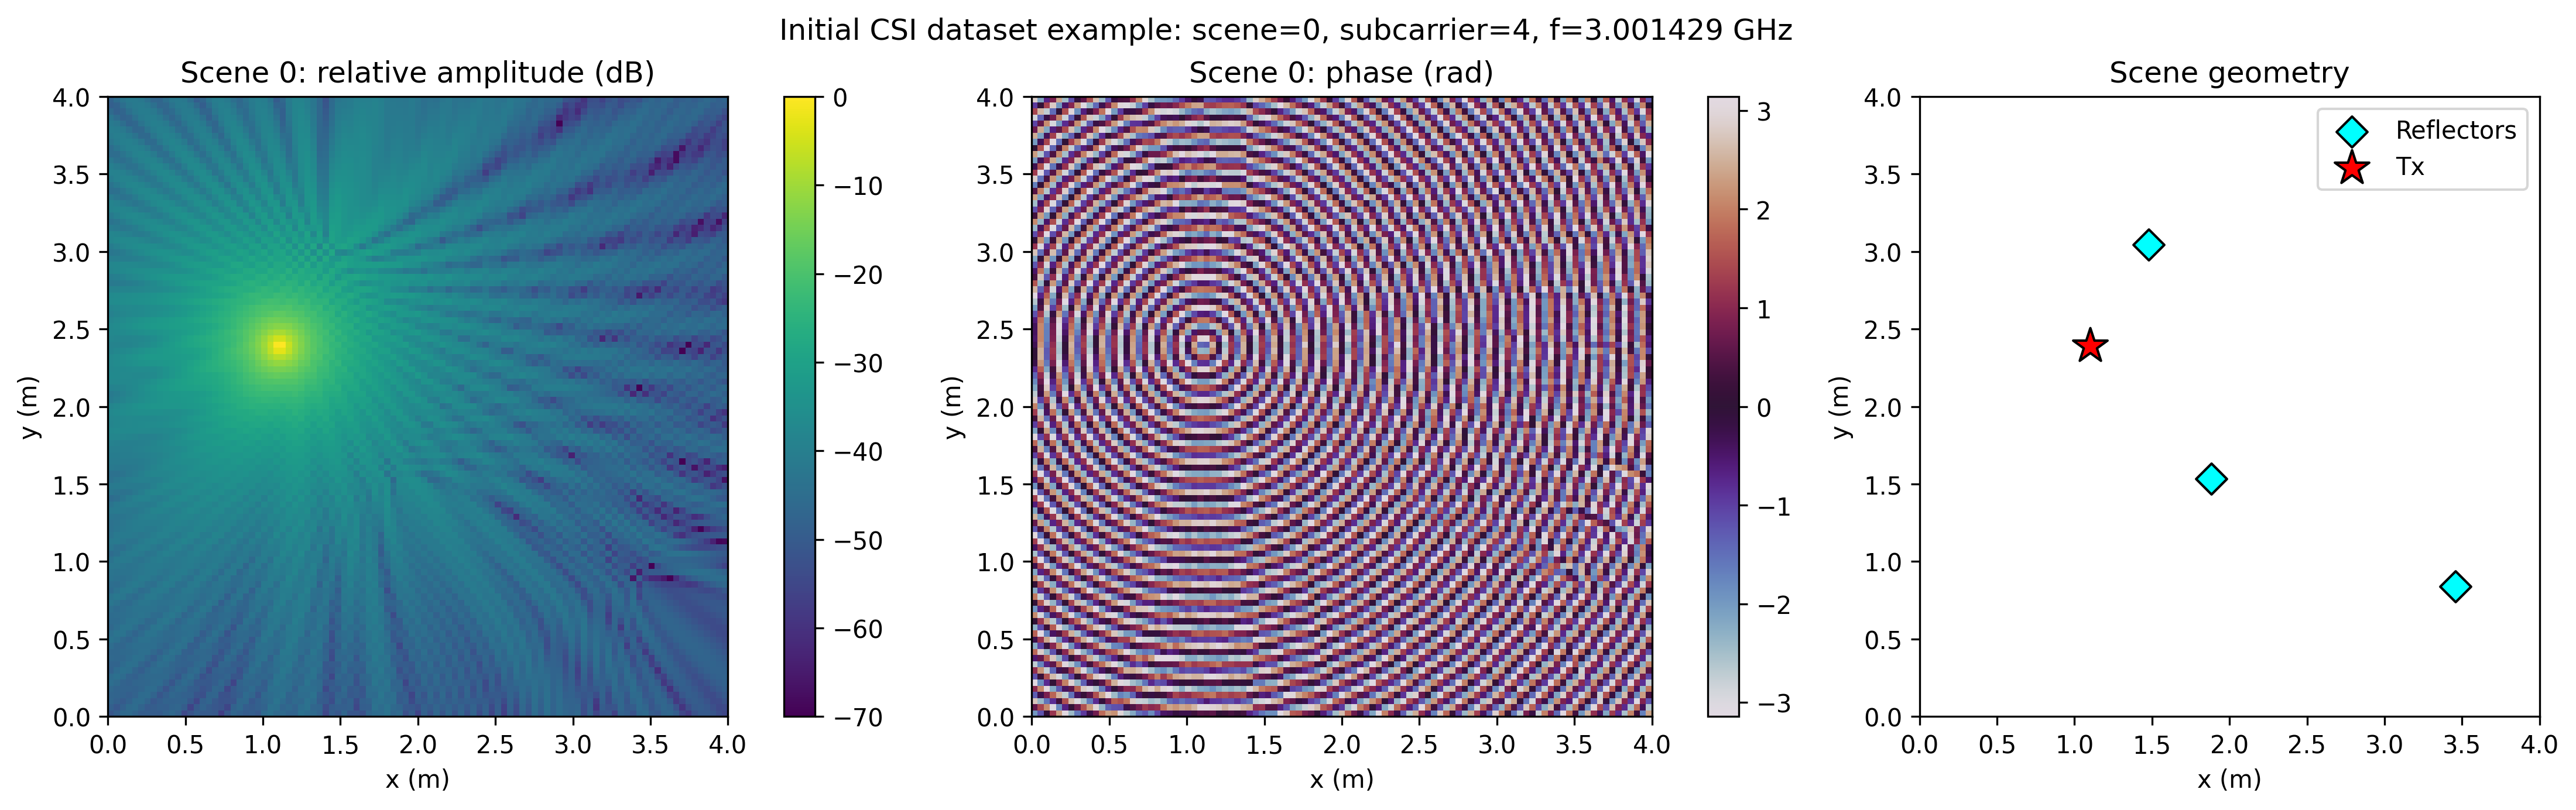
\includegraphics[width=0.98\textwidth]{initial_dataset_scene0_overview.png}
    \caption{初始数据集中场景 0 的幅度、相位与几何结构。}
    \label{fig:overview}
\end{figure}

图~\ref{fig:subcarriers} 比较同一场景中的四个子载波。
不同子载波共享相同传播几何，但传播相位中的频率 $f_k$ 不同，因此复数 CSI 及干涉条纹随子载波变化。

\begin{figure}[H]
    \centering
    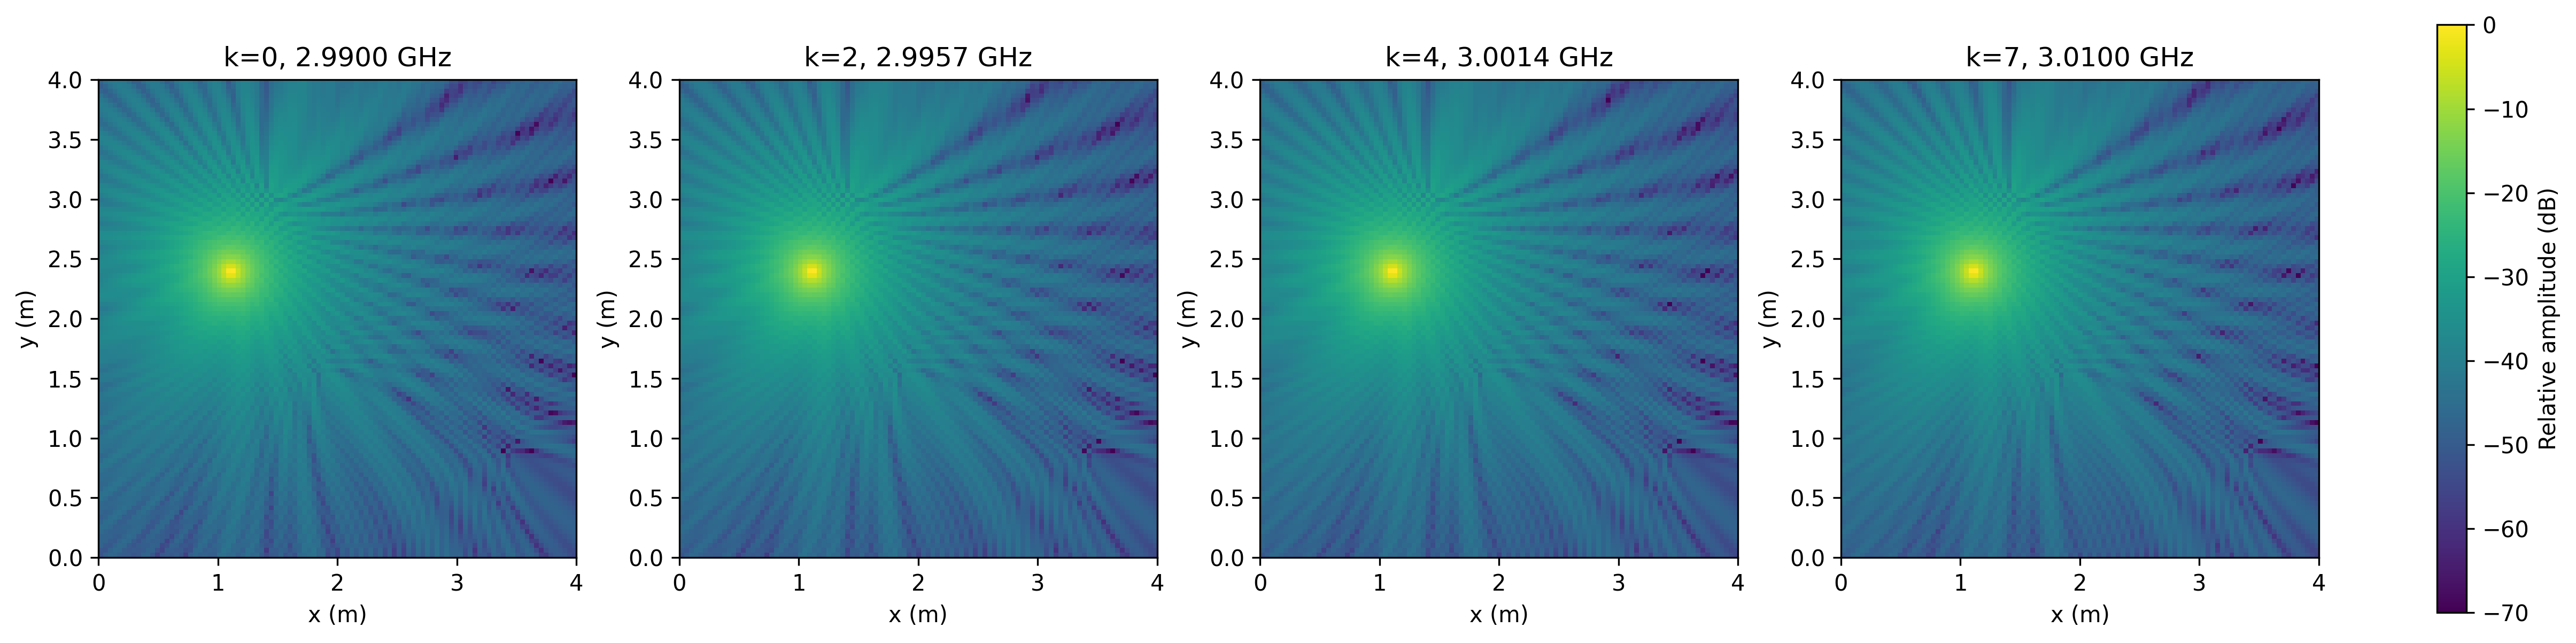
\includegraphics[width=0.98\textwidth]{initial_dataset_subcarrier_diversity.png}
    \caption{场景 0 在不同子载波上的相对幅度地图。}
    \label{fig:subcarriers}
\end{figure}

\section{稀疏测量插值 Baseline}

\subsection{实验前预测}

\textbf{我准备改变什么？}
固定数据集、测试场景和复数线性插值方法，只将随机测量位置的比例从 $5\%$ 依次增加到 $10\%$ 和 $20\%$。一个空间位置被选中后，提供该位置全部 8 个子载波的复数 CSI。

\textbf{我预计结果会如何变化？}
预计随着测量比例增加，复数 NMSE、幅度 NMAE 和相位 MAE 都会下降，其中幅度指标的改善可能比相位指标更加明显。

\textbf{为什么？}
增加测量位置可以缩小未知位置与附近已知位置之间的空间间隔，使线性插值获得更充分的局部信息；但由于 CSI 相位随传播距离快速旋转，相位误差预计仍高于幅度误差。

“提高采样率会降低三项误差”这一核心预测已在首次正式实验运行前写入 Overleaf，并通过历史编辑记录保留；本版只把方法名称收敛为最终采用的复数线性插值。实验结果与判断在后文单独补充。

\subsection{Baseline 方法与实验设置}

本文只采用一种无需训练的正式 baseline：\textbf{复数线性插值}。程序对 8 个子载波的实部和虚部分别进行二维线性插值，再组合为复数 CSI：
\begin{equation}
    \hat H_k(\mathbf p)=
    \widehat{\operatorname{Re}\{H_k(\mathbf p)\}}
    +j\widehat{\operatorname{Im}\{H_k(\mathbf p)\}}.
\end{equation}
对于线性插值无法覆盖的边界位置，使用最近测量位置的 CSI 补充。该操作只作为边界处理，不作为独立对比方法。

正式实验只在独立测试场景 $\{6,8\}$ 上运行。每次从有效空间位置中均匀随机选择 $5\%$、$10\%$ 或 $20\%$；每个场景、每个采样率使用 5 个固定随机种子，因此每个采样率共有 10 次结果。所有误差只在未观测且有效的位置计算，三种采样率使用相同的数据、代码与统计规则。

\subsection{评价指标}

本文只保留三个互补指标。复数 NMSE 是主要指标：
\begin{equation}
    \mathrm{NMSE}_{\mathrm{dB}}=
    10\log_{10}
    \frac{\sum_{\mathbf p,k}|\hat H_k(\mathbf p)-H_k(\mathbf p)|^2}
    {\sum_{\mathbf p,k}|H_k(\mathbf p)|^2}.
\end{equation}
它同时反映实部和虚部误差，数值越低越好。幅度 NMAE 定义为
\begin{equation}
    \mathrm{Amplitude\ NMAE}=
    \frac{\sum_{\mathbf p,k}\bigl||\hat H_k(\mathbf p)|-|H_k(\mathbf p)|\bigr|}
    {\sum_{\mathbf p,k}|H_k(\mathbf p)|},
\end{equation}
用于单独评价信号强度。圆周相位 MAE 定义为
\begin{equation}
    \mathrm{Phase\ MAE}=
    \frac{1}{N}\sum_{\mathbf p,k}
    \left|\angle\!\left(\hat H_k(\mathbf p)H_k^*(\mathbf p)\right)\right|,
\end{equation}
用于避免 $-\pi$ 与 $\pi$ 边界造成的普通相减错误，单位为弧度。三个指标均为越低越好。

\subsection{定量结果}

表~\ref{tab:baseline-results} 报告 8 个子载波联合计算后，在 10 次实验上的均值和标准差。

\begin{table}[H]
    \centering
    \small
    \caption{复数线性插值 baseline 的测试结果（均值 $\pm$ 标准差）}
    \label{tab:baseline-results}
    \begin{tabular}{cccc}
        \toprule
        采样率 & 复数 NMSE (dB) & 幅度 NMAE & 相位 MAE (rad) \\
        \midrule
        $5\%$  & $1.918\pm0.181$ & $0.371\pm0.024$ & $1.630\pm0.004$ \\
        $10\%$ & $2.007\pm0.146$ & $0.372\pm0.020$ & $1.677\pm0.004$ \\
        $20\%$ & $1.997\pm0.167$ & $0.385\pm0.009$ & $1.746\pm0.005$ \\
        \bottomrule
    \end{tabular}%
\end{table}

\subsection{定量与可视化结果}

图~\ref{fig:baseline-curves} 显示，复数 NMSE 始终约为 $2\,\mathrm{dB}$，没有随采样率提高而下降。幅度 NMAE 从 $0.371$ 增至 $0.385$，相位 MAE 从 $1.630\,\mathrm{rad}$ 增至 $1.746\,\mathrm{rad}$，两者反而略有变差。

\begin{figure}[H]
    \centering
    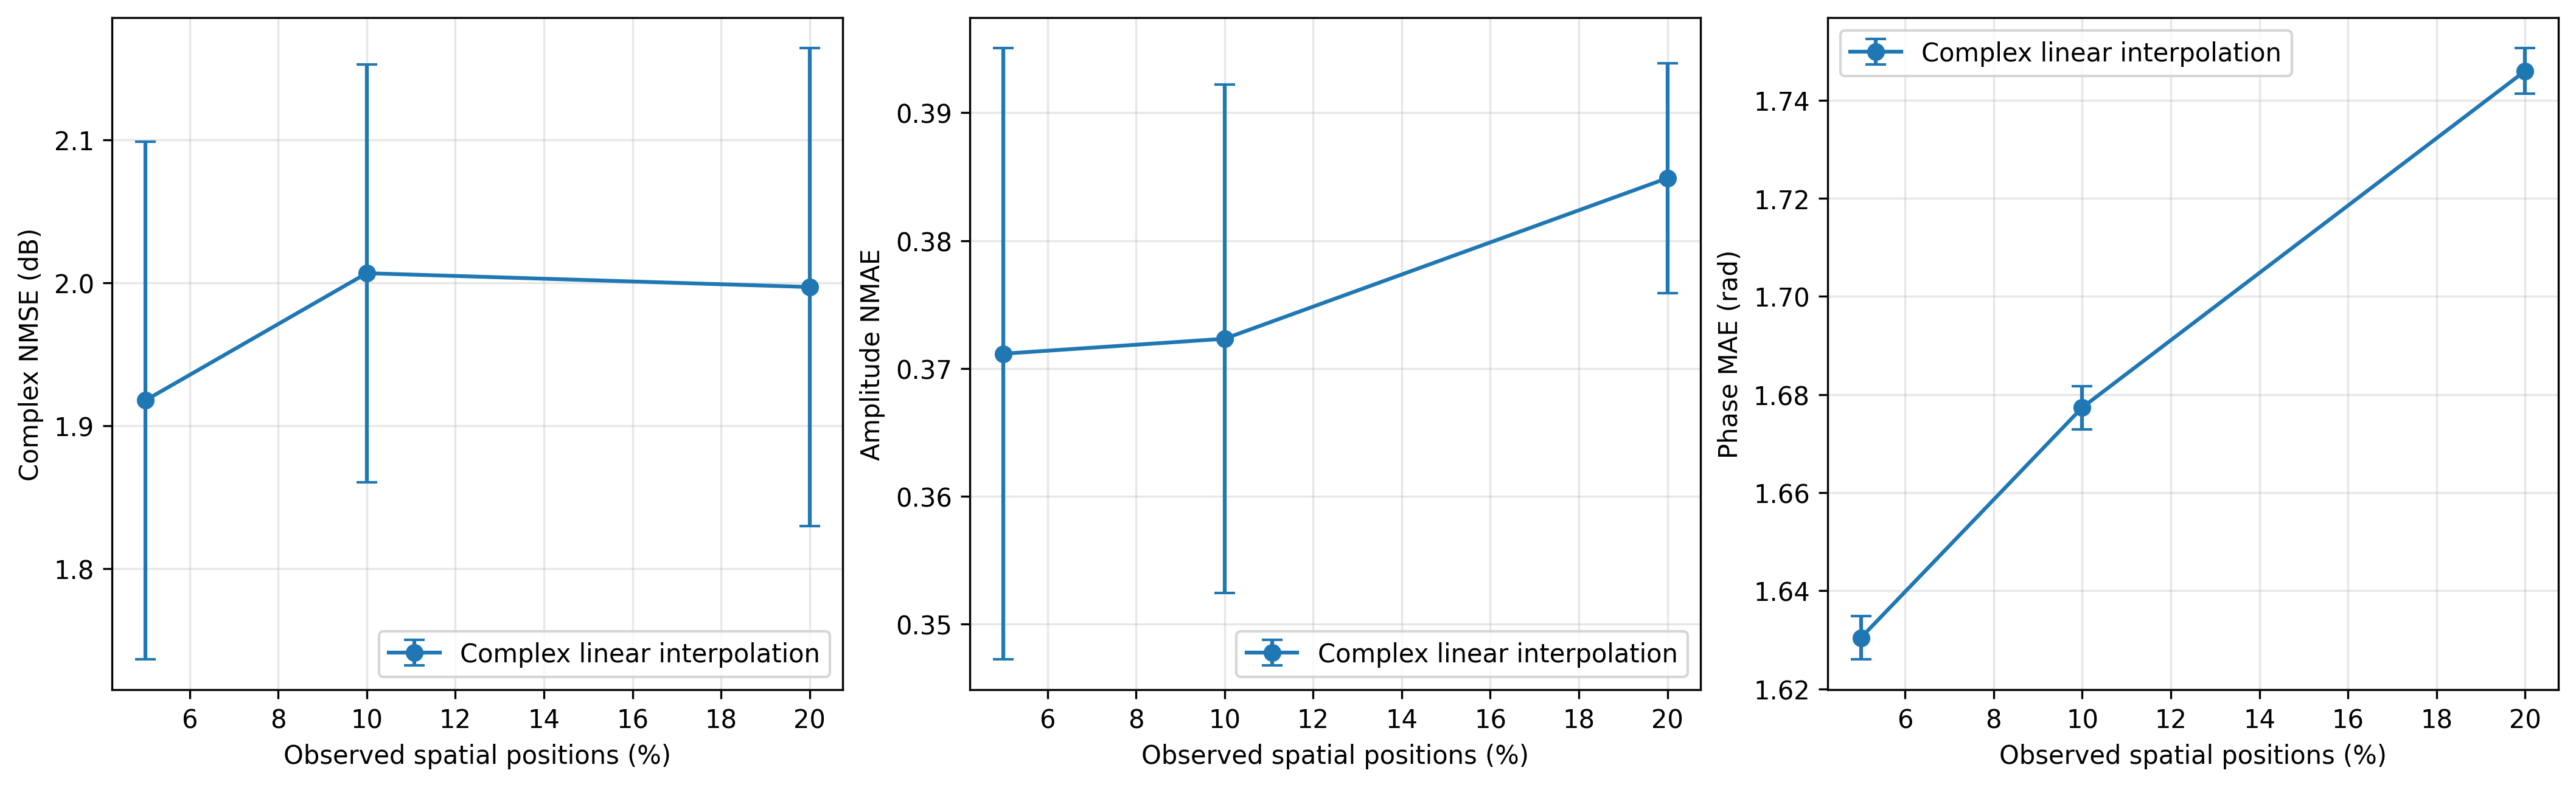
\includegraphics[width=0.88\textwidth]{baseline_metric_curves.png}
    \caption{复数线性插值在不同随机采样率下的三个测试指标。误差棒表示跨测试场景与随机重复的标准差。}
    \label{fig:baseline-curves}
\end{figure}

图~\ref{fig:baseline-reconstruction} 给出测试场景 6、第 4 个子载波在 $10\%$ 测量下的一次重建。
线性插值能够粗略定位发射机附近的强信号区域，但没有恢复真值中的细密幅度干涉条纹。其相位图只形成较大的局部色块，无法重建真实相位的密集环状变化。

\begin{figure}[H]
    \centering
    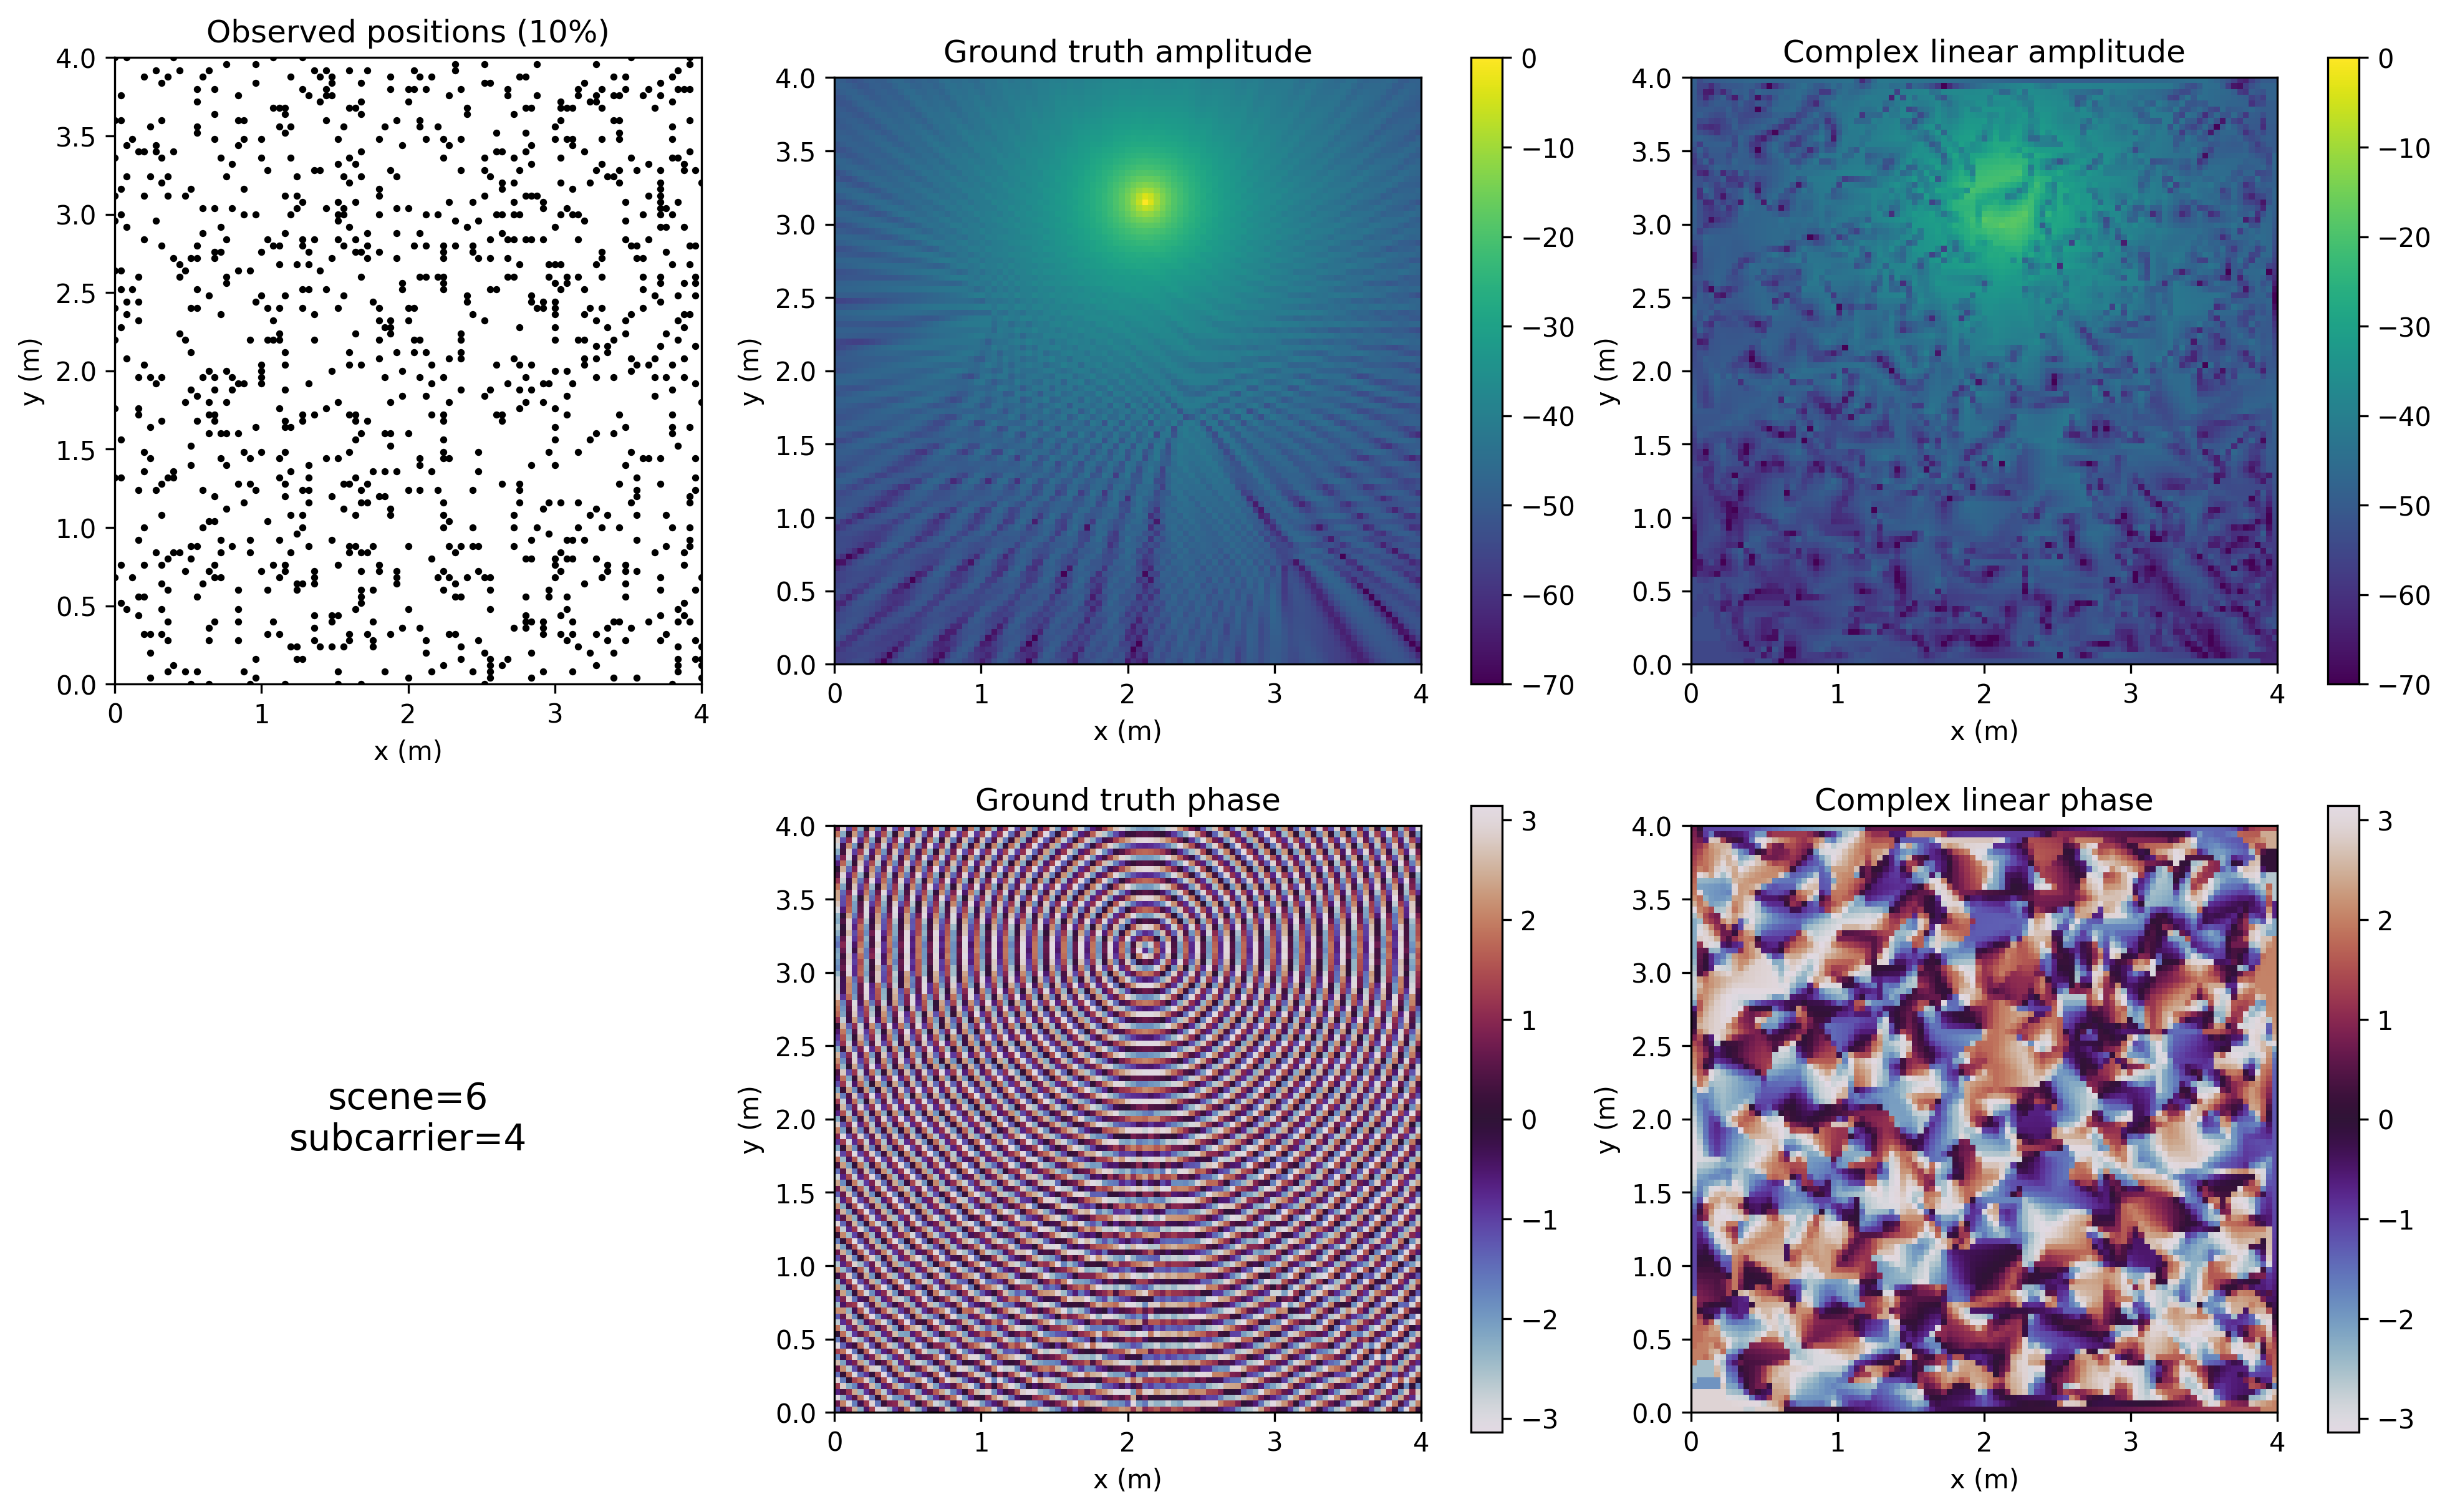
\includegraphics[width=0.99\textwidth]{baseline_10pct_reconstruction.png}
    \caption{测试场景 6、第 4 个子载波在 $10\%$ 随机空间测量下的复数线性插值重建。}
    \label{fig:baseline-reconstruction}
\end{figure}

\subsection{预测核对与失败原因}

\textbf{预测是否正确？}预测不正确。三个指标均没有随着测量比例增加而下降。程序自检能够以 $5.96\times10^{-8}$ 的最大误差恢复仿射复数场，30 条正式结果也均无 NaN 或无穷值，因此该现象不是明显的插值实现或结果汇总错误。

失败的主要原因是载波波长约为 $0.1\,\mathrm m$，而网格间距为 $0.04\,\mathrm m$。沿传播方向移动一个网格时，单径相位最多可变化约
\begin{equation}
    2\pi\frac{0.04}{0.1}\approx2.51\ \mathrm{rad}.
\end{equation}
因此，即使空间位置相邻，其复数 CSI 也可能具有接近相反的相位。线性插值对多个相位差较大的复数求加权平均时会发生相消，从而同时破坏幅度与相位。

这个结果说明，完整 $101\times101$ 网格满足半波长条件，并不代表从中随机保留 $20\%$ 后仍满足相位重建所需的有效采样条件。
复数线性插值没有使用波数、传播距离或跨场景先验，因此增加少量随机点不一定单调改善复数 CSI。本实验作为效果较差的实验被保留，并说明后续改进方法必须显式利用空间频率或传播结构。

\section{AI 建议的审计与人工判断}

AI 助手最初建议使用 $64\times64$ 网格，以降低计算量。该建议最终没有采用，因为它忽略了载波波长对空间采样密度的约束。

在最高频率 $3.01\,\mathrm{GHz}$ 下，最短波长约为
\begin{equation}
    \lambda_{\min}=\frac{c}{f_{\max}}=0.09967\,\mathrm m,
\end{equation}
半波长约为 $0.04983\,\mathrm m$。$64\times64$ 网格在 $4\,\mathrm m$ 区域中的间距为
\begin{equation}
    \Delta x_{64}=\frac{4}{63}=0.06349\,\mathrm m,
\end{equation}
大于半波长，会对快速空间相位变化产生混叠。实际生成的相位图也出现明显棋盘状伪影。

本文通过两种方法判断原建议存在问题：第一，计算网格间距并与最高载波频率对应的半波长比较；第二，对生成相位图进行可视化检查。
随后将网格提高到 $101\times101$，使间距降至 $0.04\,\mathrm m$，并把半波长条件加入生成脚本的自动断言。
这说明 AI 给出的计算规模建议不能直接采用，必须结合电磁波长和可视化结果验证。

\subsection{Fourier-feature MLP}

\textbf{我准备改变什么？}
保持数据集、$5\%$、$10\%$、$20\%$ 测量位置、随机种子、未观测评价位置和三个指标完全不变，只将预测方法从复数线性插值改为 Fourier-feature MLP。模型把归一化二维坐标映射为多组正弦和余弦特征，再一次输出 8 个子载波的实部与虚部。模型设置只在验证场景 1 和 7 上选择，测试场景 6 和 8 不参与调参。

\textbf{我预计结果会如何变化？}
预计 Fourier-feature MLP 在 $10\%$ 和 $20\%$ 测量下可以降低复数 NMSE 和相位 MAE，因为它能够表示线性插值无法恢复的高频空间变化。幅度 NMAE 预计也会降低，但改善可能小于复数 NMSE。在 $5\%$ 测量下，观测可能不足，模型存在过拟合风险，因此不保证明显优于线性插值。

\textbf{为什么？}
复数线性插值只根据局部几何权重平均测量值，相位差较大时会产生复数相消。Fourier 坐标特征显式提供不同空间频率的正弦和余弦基函数，使小型 MLP 更容易拟合约 $0.1\,\mathrm m$ 波长产生的快速相位旋转\cite{fourierfeatures}。另一方面，过高的 Fourier 频率也可能只记住稀疏测量点，因此将使用测量点内部验证和早停控制过拟合。

\textbf{判断标准：}
仍以复数 NMSE 为主要指标，并结合幅度 NMAE 和相位 MAE。若 Fourier-feature MLP 在相同采样掩码下取得更低的平均复数 NMSE，且相位 MAE 没有明显恶化，则认为改进有效。

\subsection{实现与验证集选择}

模型输入为二维物理坐标 $(x,y)$，先经过 6 组空间频率和 8 个方向构成的正弦、余弦编码，再通过 3 层、每层 128 个单元的 ReLU MLP，一次输出 8 个子载波的实部和虚部，共 16 维。训练损失为归一化实部、虚部均方误差。

每次从测量位置中保留 $20\%$ 作为内部早停集合，选择最佳训练轮数后，再使用全部测量位置重新训练相同轮数。最大 Fourier 频率的候选值为 4、8 和 12 cycles/m，只在验证场景 1 和 7 的 $10\%$ 测量条件下选择。三者验证集平均复数 NMSE 分别为 $0.0158$、$0.0113$ 和 $0.0104\,\mathrm{dB}$，因此按预定主指标选择 12 cycles/m。三者差异很小，说明仅改变最大 Fourier 频率没有实质解决泛化问题。

\subsection{实验结果}

表~\ref{tab:fourier-mlp-results} 给出复数线性插值和 Fourier MLP 在完全相同测量掩码下的结果。

\begin{table}[H]
    \centering
    \small
    \caption{复数线性插值与 Fourier MLP 的测试结果（均值 $\pm$ 标准差）}
    \label{tab:fourier-mlp-results}
    \begin{tabular}{ccccc}
        \toprule
        采样率 & 方法 & 复数 NMSE (dB) & 幅度 NMAE & 相位 MAE (rad) \\
        \midrule
        $5\%$  & 复数线性插值 & $1.918\pm0.181$ & $0.371\pm0.024$ & $1.630\pm0.004$ \\
        $5\%$  & Fourier MLP   & $0.022\pm0.031$ & $0.906\pm0.052$ & $1.561\pm0.009$ \\
        $10\%$ & 复数线性插值 & $2.007\pm0.146$ & $0.372\pm0.020$ & $1.677\pm0.004$ \\
        $10\%$ & Fourier MLP   & $0.015\pm0.016$ & $0.907\pm0.032$ & $1.554\pm0.017$ \\
        $20\%$ & 复数线性插值 & $1.997\pm0.167$ & $0.385\pm0.009$ & $1.746\pm0.005$ \\
        $20\%$ & Fourier MLP   & $0.004\pm0.010$ & $0.904\pm0.041$ & $1.533\pm0.034$ \\
        \bottomrule
    \end{tabular}
\end{table}

\begin{figure}[H]
    \centering
    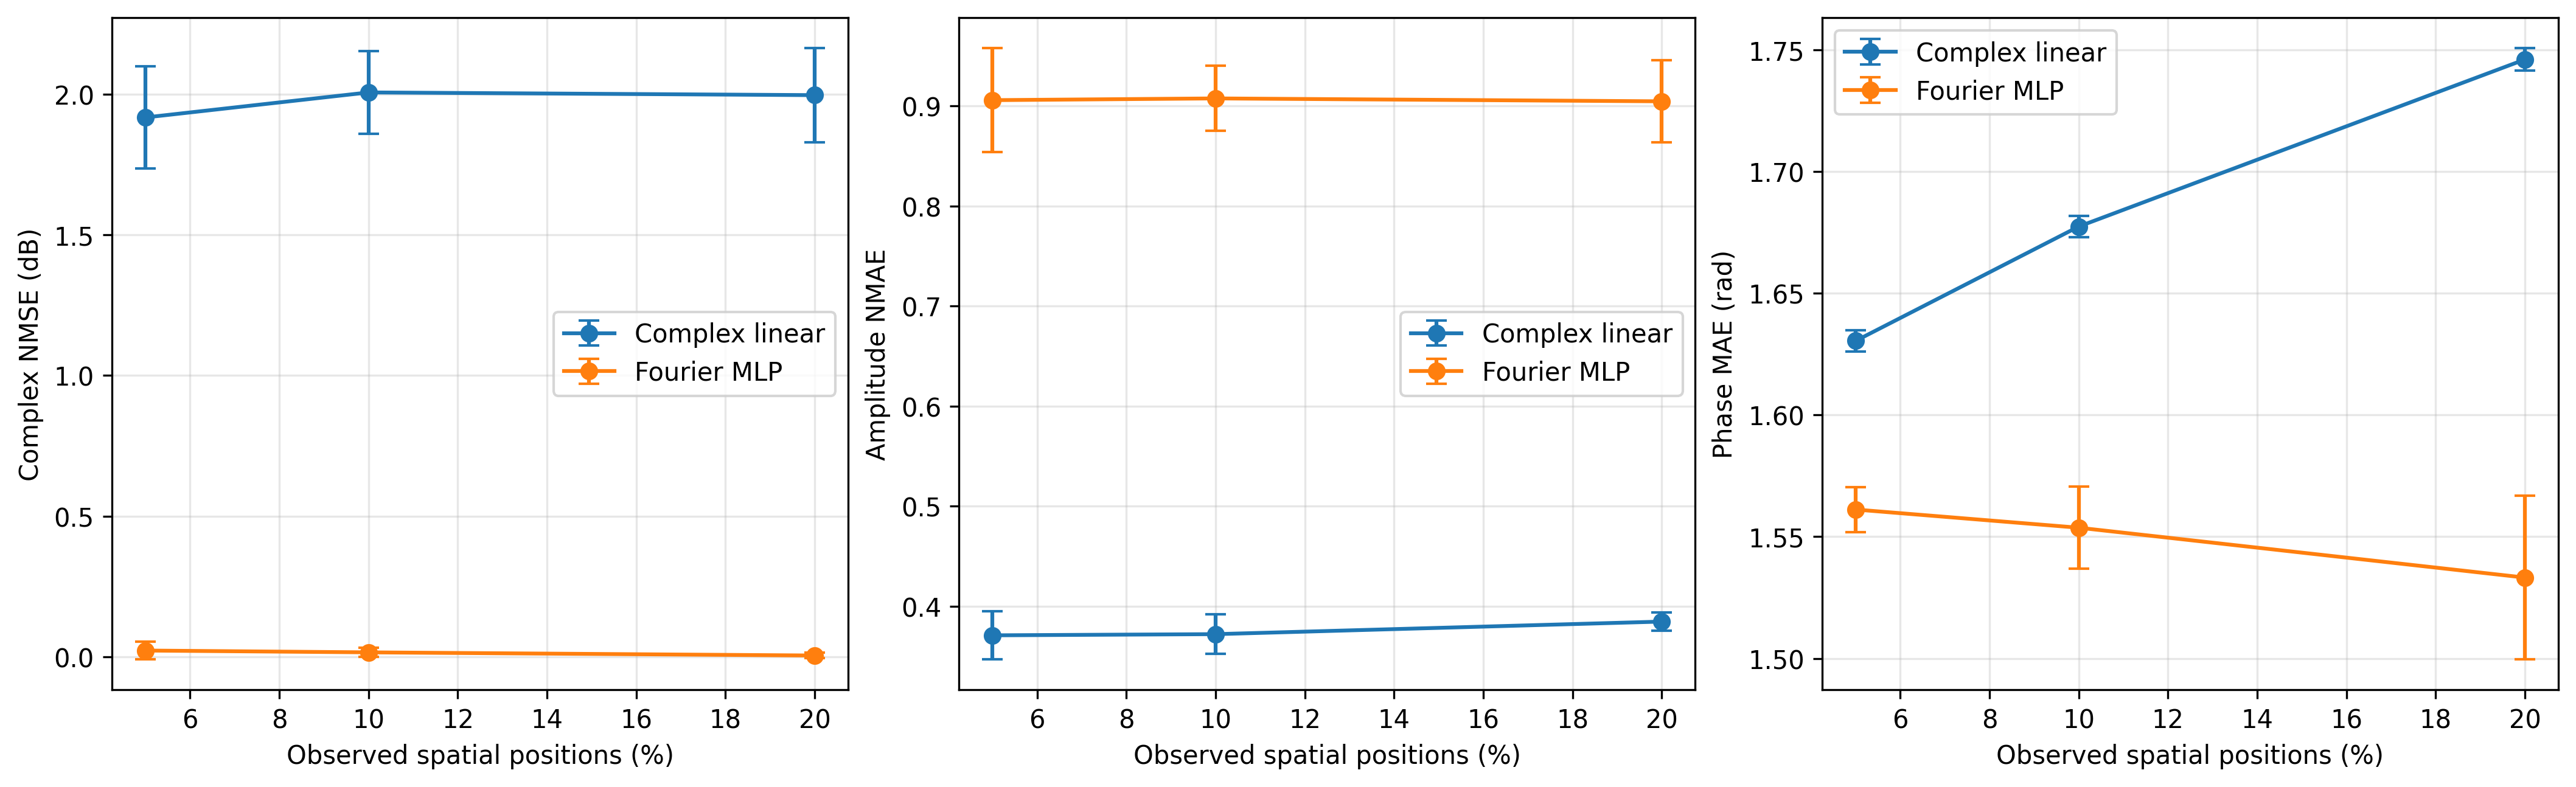
\includegraphics[width=0.96\textwidth]{fourier_mlp_comparison_curves.png}
    \caption{复数线性插值与 Fourier MLP 的三个测试指标。}
    \label{fig:fourier-mlp-curves}
\end{figure}

\begin{figure}[H]
    \centering
    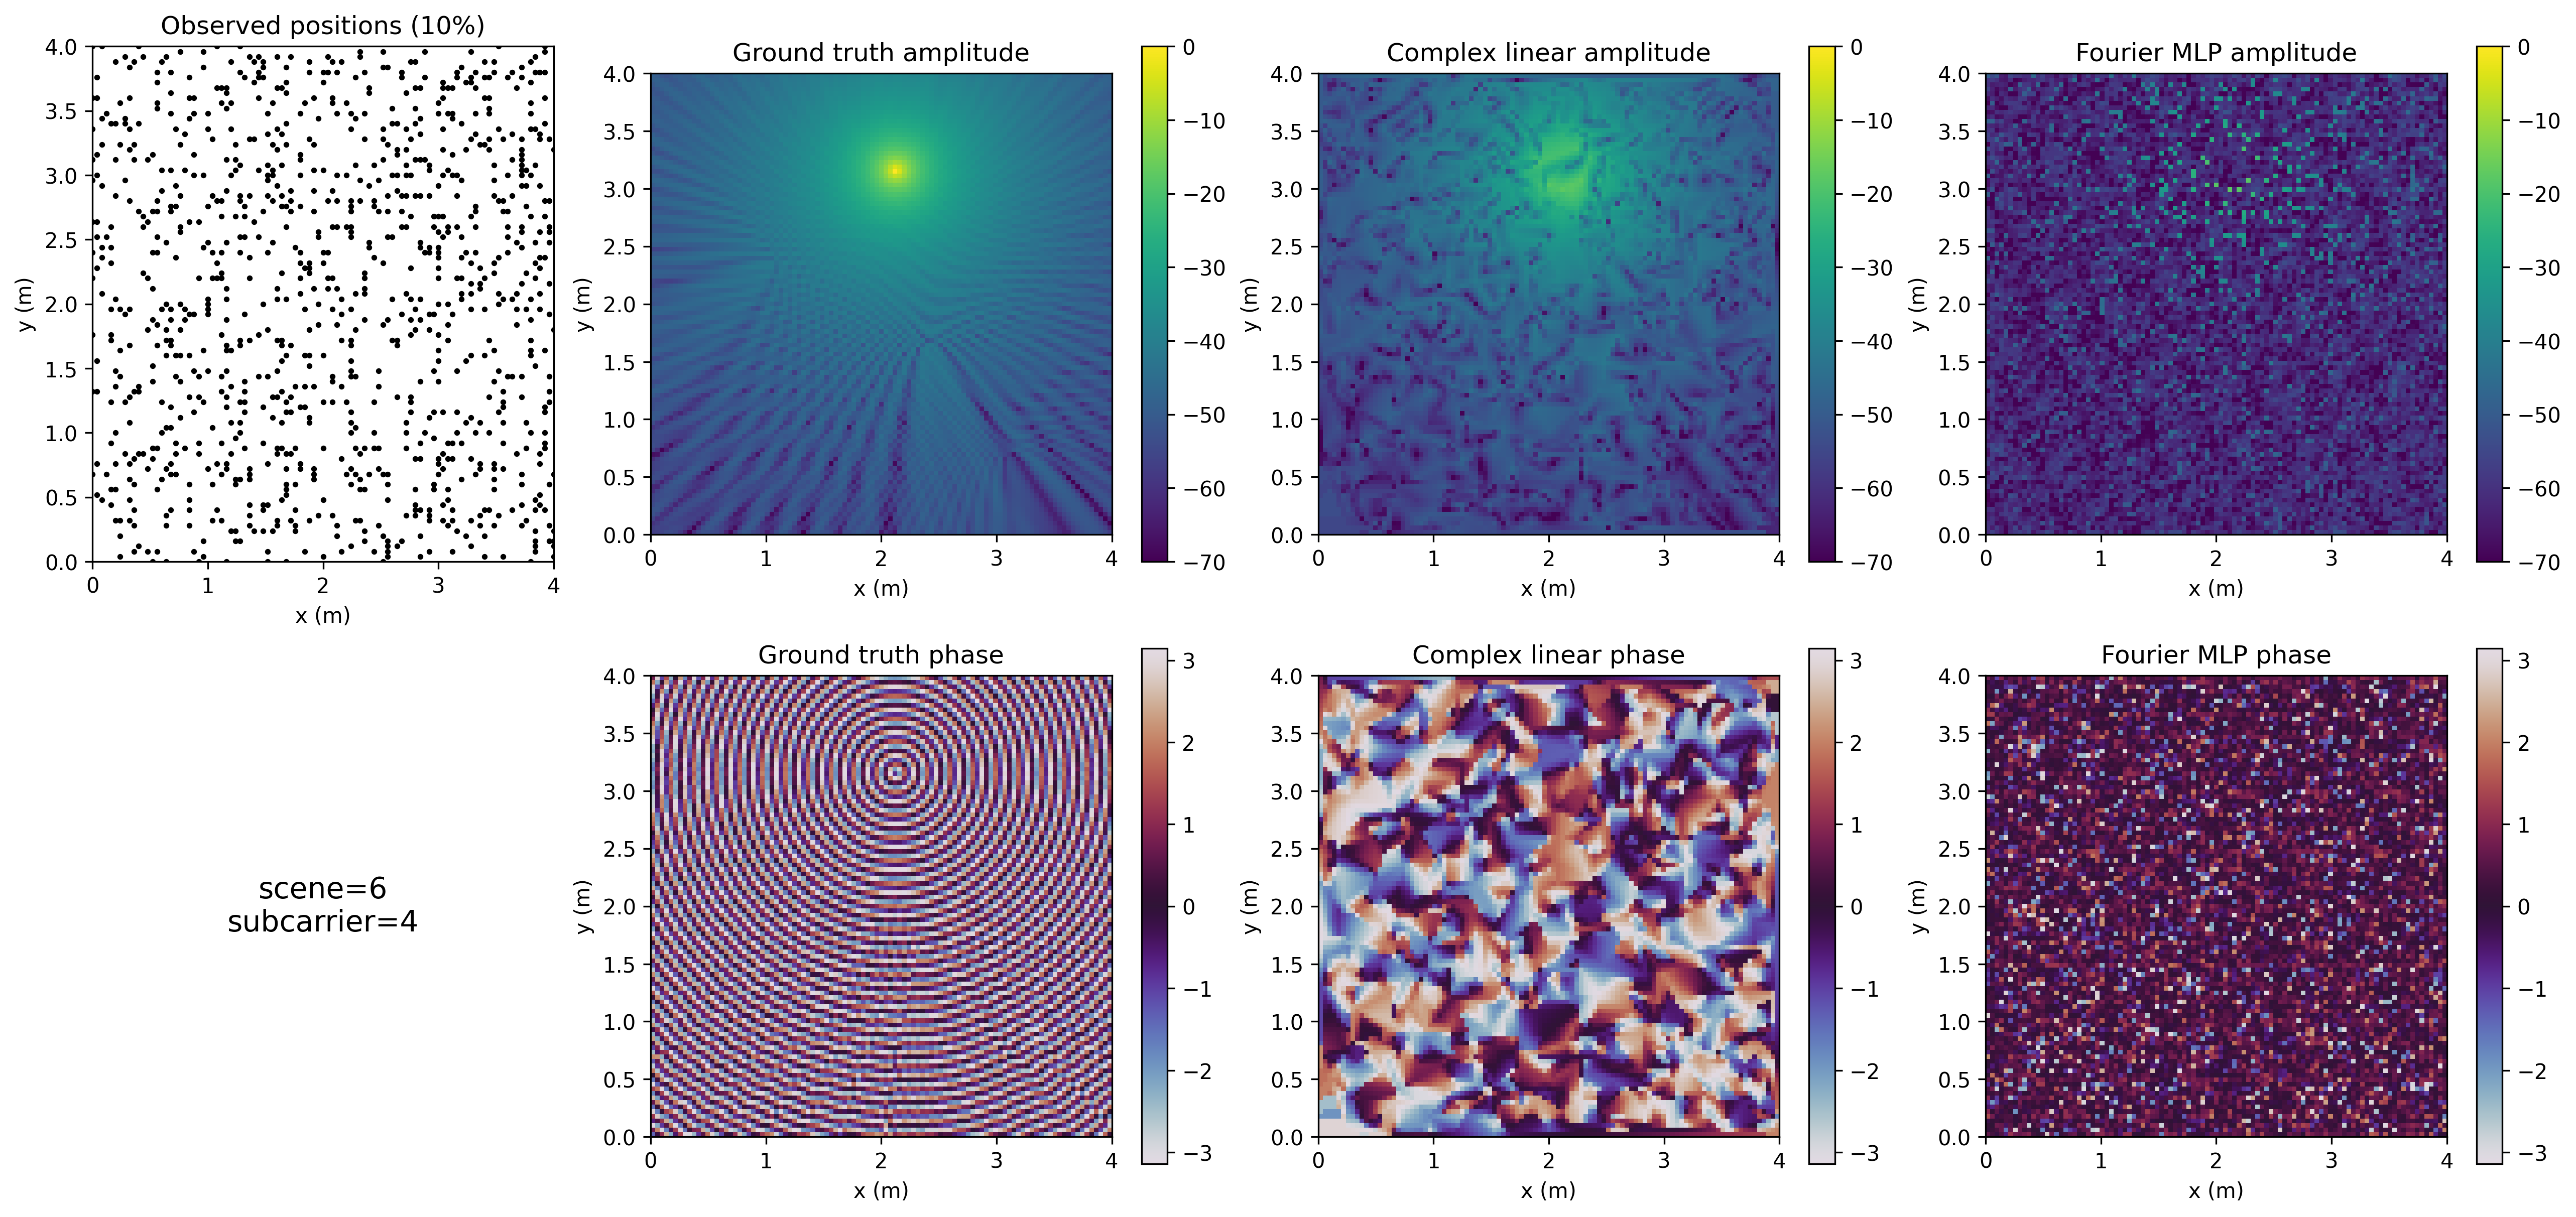
\includegraphics[width=0.99\textwidth]{fourier_mlp_10pct_reconstruction.png}
    \caption{测试场景 6、第 4 个子载波在 $10\%$ 测量下的重建对比。}
    \label{fig:fourier-mlp-reconstruction}
\end{figure}

\subsection{预测核对与失败分析}

Fourier MLP 的复数 NMSE 数值从约 $2\,\mathrm{dB}$ 降至接近 $0\,\mathrm{dB}$，相位 MAE 也略低于线性插值，但这并不代表模型有效恢复了 CSI。若所有未知位置均预测为零，则
\begin{equation}
    \mathrm{NMSE}=
    \frac{\sum|0-H|^2}{\sum|H|^2}=1,
    \qquad
    \mathrm{NMSE}_{\mathrm{dB}}=0\,\mathrm{dB}.
\end{equation}
本实验中 Fourier MLP 的幅度 NMAE 高达 $0.904$--$0.907$，非常接近零预测对应的 1；相位 MAE 为 $1.533$--$1.561\,\mathrm{rad}$，也接近随机相位参考值 $\pi/2\approx1.571\,\mathrm{rad}$。图~\ref{fig:fourier-mlp-reconstruction} 进一步显示，模型在大部分未知区域输出接近零的幅度，并未恢复发射机附近的连续衰减或密集相位环。

测量点内部早停选择的轮数只有 2--17 轮，平均为 8.47 轮。说明网络继续拟合测量点时，内部验证误差很快上升，早停最终保留了接近初始化、输出接近零的模型。其原因是稀疏位置上的复数相位变化过快，固定平面波 Fourier 特征并没有提供场景中的发射机距离和多径路径结构，网络难以从少量随机位置推断正确相位。对于均方误差而言，在相位无法预测时输出接近零反而比输出错误相位的非零信号具有更低损失。

因此，实验前预测只在 NMSE 和相位 MAE 的表面数值上成立，关于“模型恢复了高频 CSI”的核心假设不成立，幅度改善预测也完全错误。该结果同时说明原判断标准不够充分：必须联合检查幅度 NMAE 和重建图，不能只根据 NMSE 排名宣布改进成功。本实验作为效果较差的实验保留。

\subsubsection{基于失败分析的后续改进假设}

普通 Fourier MLP 的失败表明，仅增加通用高频坐标特征不足以推断场景相关传播相位。下一步保留相同网络、采样掩码和评价指标，只加入已知 Tx 位置和子载波频率构成的直达径相位补偿。令
\begin{equation}
    d_0(\mathbf p)=\|\mathbf p-\mathbf p_{\mathrm{Tx}}\|_2,
\end{equation}
并将训练目标变换为
\begin{equation}
    Z_k(\mathbf p)=H_k(\mathbf p)
    \exp\left(+j\frac{2\pi f_kd_0(\mathbf p)}{c}\right).
\end{equation}
模型预测 $\hat Z_k$ 后，再恢复
\begin{equation}
    \hat H_k(\mathbf p)=\hat Z_k(\mathbf p)
    \exp\left(-j\frac{2\pi f_kd_0(\mathbf p)}{c}\right).
\end{equation}

该变换能解析地去除直达径中已知的快速载波相位，使网络主要学习较平滑的幅度衰减和多径路径差。预计该方法首先会明显降低普通 Fourier MLP 约 $0.90$ 的幅度 NMAE，并避免接近零输出；在 $10\%$ 和 $20\%$ 测量下，复数 NMSE 和相位 MAE 也有望进一步改善。$5\%$ 测量下仍可能因多径残差欠采样而失败。该实验不使用真实反射点、反射系数或未观测 CSI，因此没有引入测试答案。

\subsubsection{实验结果}

相位补偿后的目标明显更加平滑。在验证场景 1 和 7 上，最大 Fourier 频率为 1、2、4、8 和 12 cycles/m 时，平均复数 NMSE 分别为 $-16.92$、$-16.03$、$-6.57$、$-2.19$ 和 $-2.20\,\mathrm{dB}$。因此只依据验证集固定选择 1 cycle/m，再一次性运行测试场景 6 和 8。普通 Fourier MLP 选择了 12 cycles/m，而相位补偿后最低候选频率表现最好，支持“物理补偿降低了待学习空间频率”的解释。

\begin{table}[H]
    \centering
    \small
    \caption{三种方法在独立测试场景上的结果（均值 $\pm$ 标准差）}
    \label{tab:tx-aware-results}
    \resizebox{\textwidth}{!}{%
    \begin{tabular}{ccccc}
        \toprule
        采样率 & 方法 & 复数 NMSE (dB) & 幅度 NMAE & 相位 MAE (rad) \\
        \midrule
        $5\%$ & 复数线性插值 & $1.918\pm0.181$ & $0.371\pm0.024$ & $1.630\pm0.004$ \\
        $5\%$ & 普通 Fourier MLP & $0.022\pm0.031$ & $0.906\pm0.052$ & $1.561\pm0.009$ \\
        $5\%$ & Tx-aware Fourier MLP & $-13.291\pm3.718$ & $0.190\pm0.055$ & $0.270\pm0.043$ \\
        \midrule
        $10\%$ & 复数线性插值 & $2.007\pm0.146$ & $0.372\pm0.020$ & $1.677\pm0.004$ \\
        $10\%$ & 普通 Fourier MLP & $0.015\pm0.016$ & $0.907\pm0.032$ & $1.554\pm0.017$ \\
        $10\%$ & Tx-aware Fourier MLP & $-14.854\pm3.851$ & $0.161\pm0.049$ & $0.248\pm0.035$ \\
        \midrule
        $20\%$ & 复数线性插值 & $1.997\pm0.167$ & $0.385\pm0.009$ & $1.746\pm0.005$ \\
        $20\%$ & 普通 Fourier MLP & $0.004\pm0.010$ & $0.904\pm0.041$ & $1.533\pm0.034$ \\
        $20\%$ & Tx-aware Fourier MLP & $-15.842\pm4.272$ & $0.147\pm0.047$ & $0.236\pm0.031$ \\
        \bottomrule
    \end{tabular}%
    }
\end{table}

\begin{figure}[H]
    \centering
    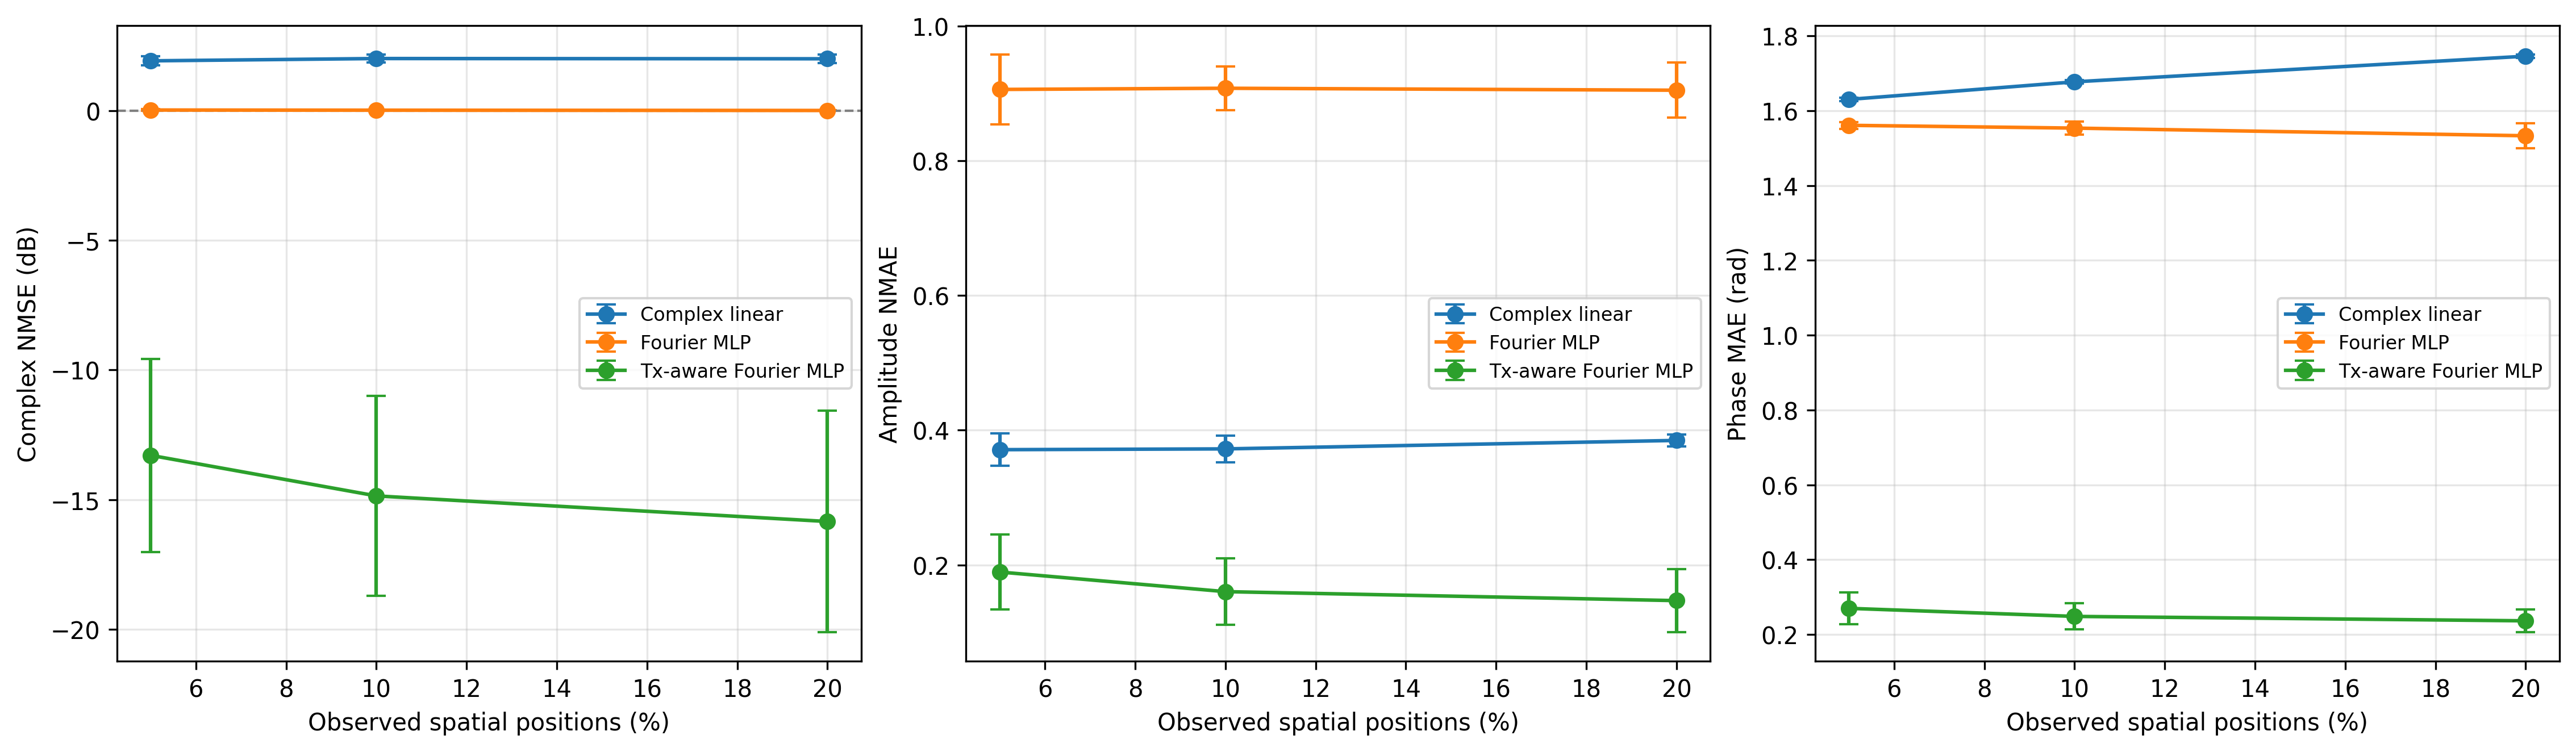
\includegraphics[width=0.98\textwidth]{tx_aware_comparison_curves.png}
    \caption{复数线性插值、普通 Fourier MLP 和 Tx-aware Fourier MLP 的测试结果。NMSE 图中的灰色虚线表示零预测对应的 $0\,\mathrm{dB}$。}
    \label{fig:tx-aware-curves}
\end{figure}

\begin{figure}[H]
    \centering
    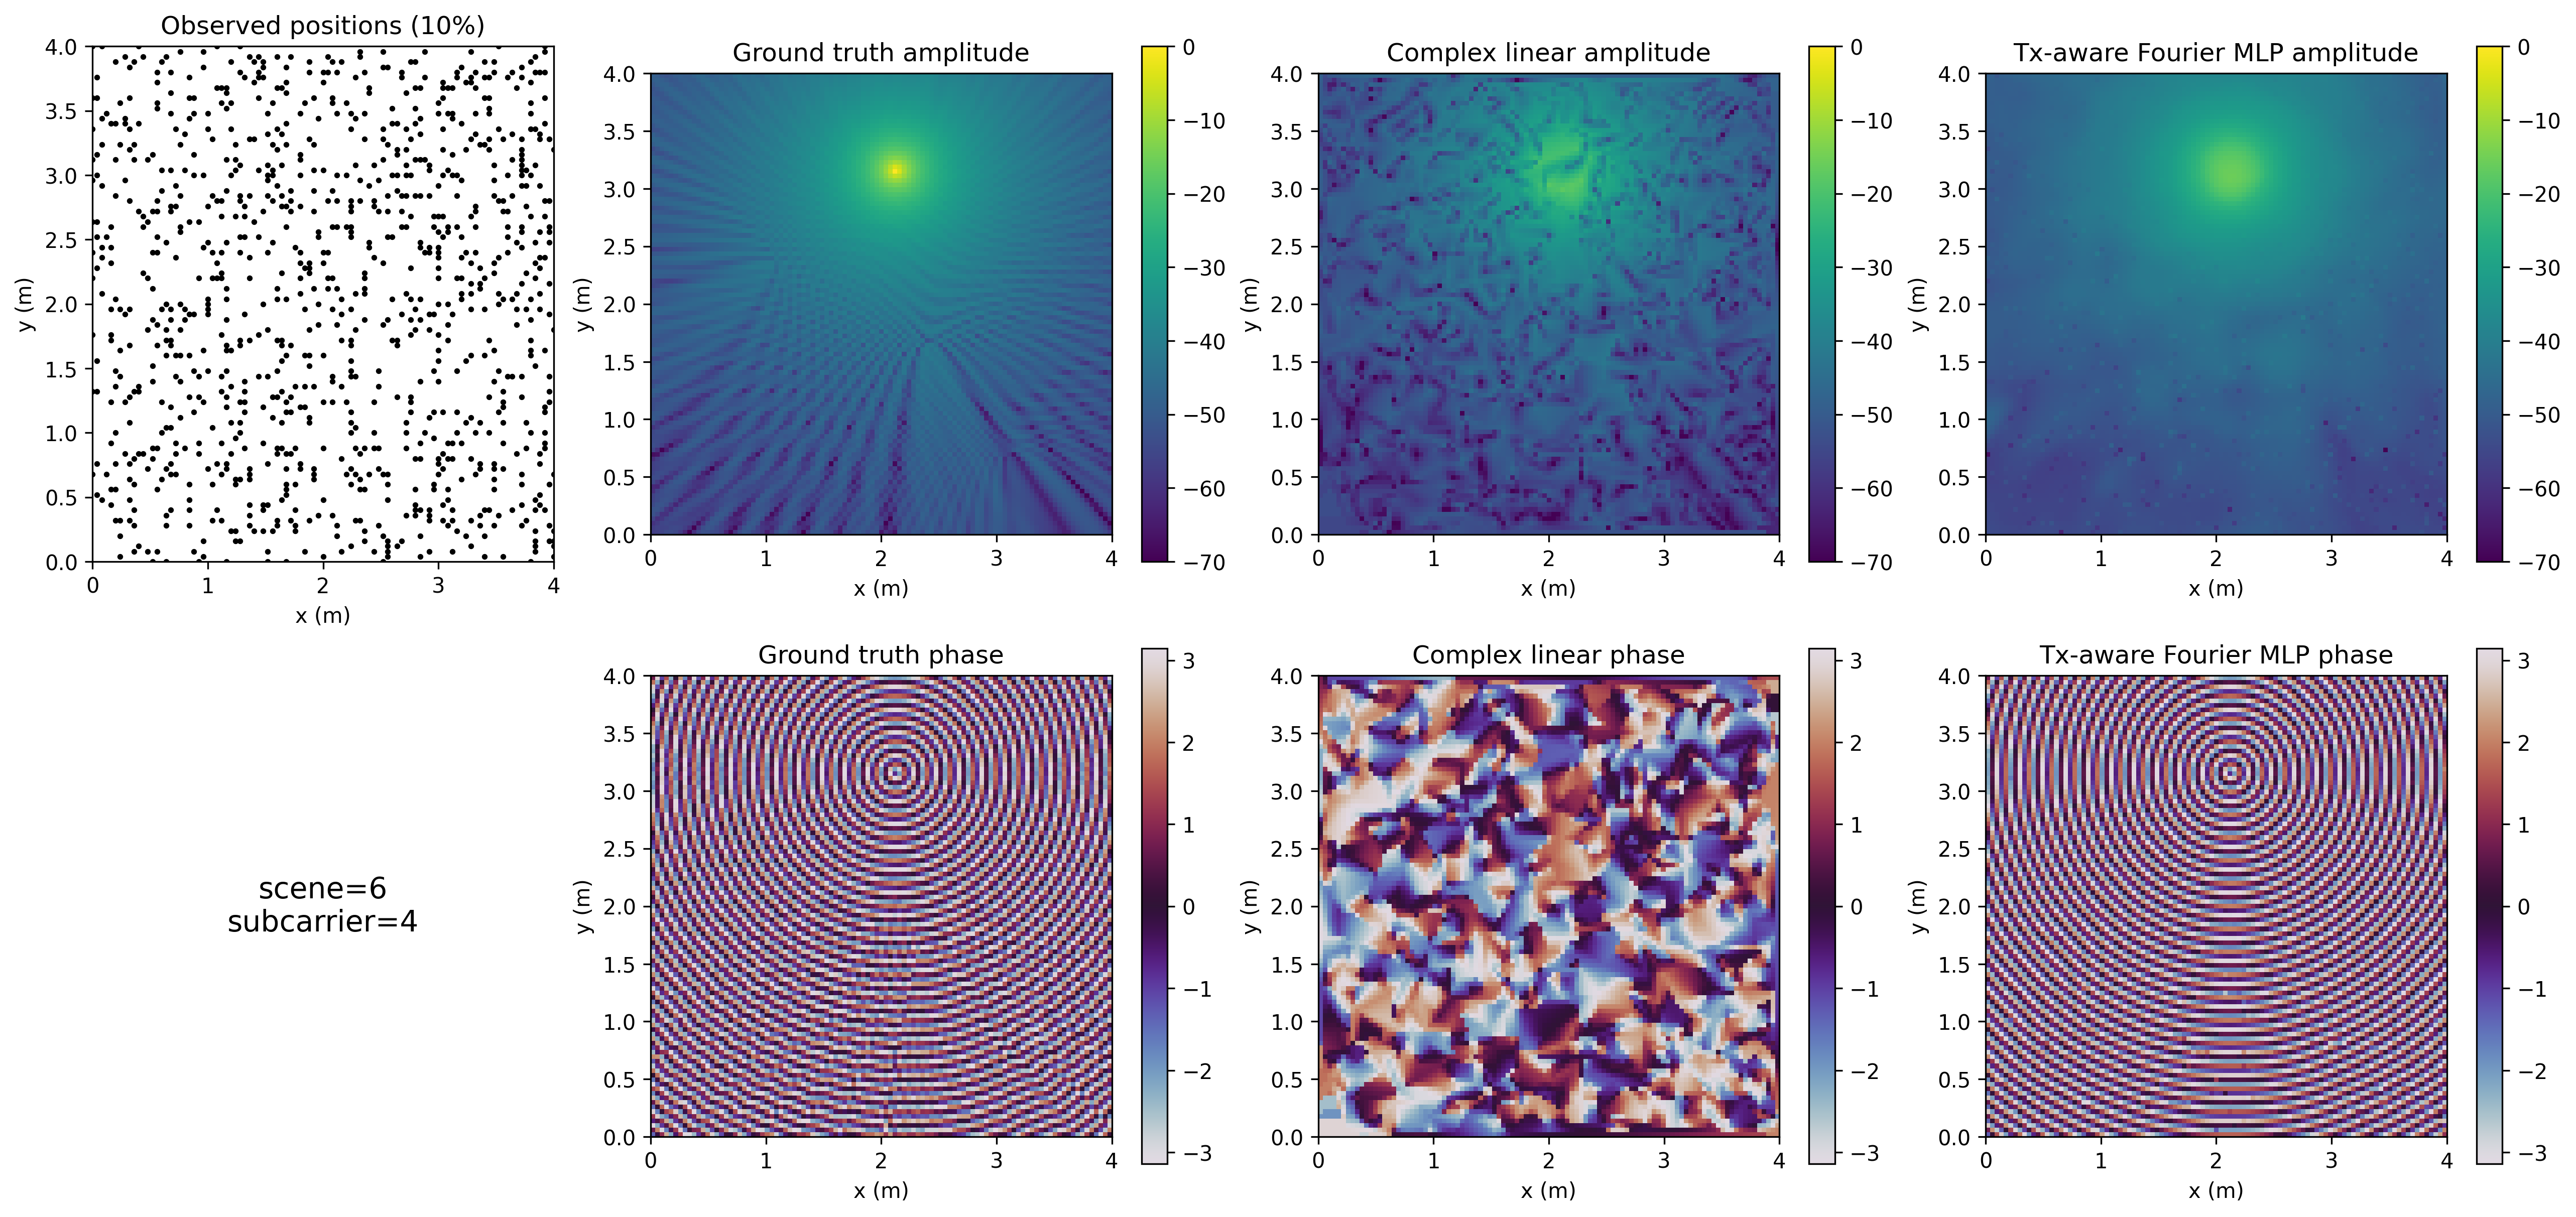
\includegraphics[width=0.99\textwidth]{tx_aware_10pct_reconstruction.png}
    \caption{测试场景 6、第 4 个子载波在 $10\%$ 测量下的 Tx-aware 重建。}
    \label{fig:tx-aware-reconstruction}
\end{figure}

\subsubsection{预测核对}

实验预测总体正确，而且 $5\%$ 测量下也获得明显改善。随着采样率从 $5\%$ 增加到 $20\%$，Tx-aware 方法的复数 NMSE 从 $-13.291$ 降至 $-15.842\,\mathrm{dB}$，幅度 NMAE 从 $0.190$ 降至 $0.147$，相位 MAE 从 $0.270$ 降至 $0.236\,\mathrm{rad}$。早停轮数从普通 Fourier MLP 的平均 8.47 轮增加到 171.3 轮，也说明补偿后的目标能够在未参与训练的测量位置上持续泛化，而不是停留在接近零初始化。

图~\ref{fig:tx-aware-reconstruction} 显示，Tx-aware 方法恢复了发射机附近的主要幅度衰减和密集相位环，但仍弱化了真值中的多径干涉条纹。需要特别说明，相位环主要由已知 Tx 距离和载波频率解析恢复，不能解释为网络独立学会了完整电磁传播。较大的 NMSE 标准差也表明不同场景的多径残差难度仍有差异。

该实验只使用实际系统中通常已知的 Tx 位置、接收位置和子载波频率，没有使用真实反射点、反射系数或未观测 CSI。尽管如此，当前合成数据与相位补偿使用相同的自由空间相位公式，因此结果属于有利条件下的验证；在存在非视距、Tx 定位误差、硬件相位偏移或时钟不同步时，性能可能下降。

\section{下一项实验的预先预测}

\subsection{改变采样空间分布}

\textbf{我准备改变什么？}
固定 $10\%$ 测量数量，比较全区域随机分散采样与局部聚集采样。

\textbf{我预计结果会如何变化？}
局部聚集采样在远离测量区域的位置具有更高误差，并且跨场景平均结果差于随机分散采样。

\textbf{为什么？}
随机测量覆盖整个空间，主要进行局部插值；聚集测量只能约束局部区域，其他区域需要长距离外推。

\textbf{真实结果：}尚未运行。

\textbf{预测是否正确：}待实验后填写。

\section{当前局限与后续计划}

当前数据仍是简化点反射模型，没有模拟建筑物遮挡、绕射、天线方向图、硬件相位偏移和测量噪声。
10 个场景适合验证数据与实验流程，但对于训练较大的 CNN 或 diffusion 模型仍然过少。

下一阶段将依次完成：
\begin{enumerate}[label=(\arabic*)]
    \item 完成固定 $10\%$ 数量下随机分散与局部聚集采样的对比；
    \item 对 Tx 位置误差、未知公共相位偏移和非视距场景进行稳健性实验；
    \item 在不使用真实反射点的前提下，将直达分量和多径残差分开建模，以恢复目前仍被平滑掉的干涉条纹；
    \item 如果需要训练更大的跨场景网络，再增加训练场景数量。
\end{enumerate}

如果继续增加三天实验时间，最优先的修改是加入未知公共相位偏移和 Tx 位置扰动的联合估计。当前方法的主要增益来自精确直达径相位补偿，而真实 CSI 往往包含硬件、同步和定位误差。若不验证这种模型失配，当前优秀结果可能只适用于理想合成数据。随后再将直达分量与多径残差分开建模，以改善仍未恢复的干涉细节。

\section{结论}

本文完成了任务 D 的数据基础：生成包含 10 个场景、8 个子载波、每场景一条直达径和三条反射径的复数 CSI 数据集。
数据通过了数值完整性、场景差异、子载波差异和空间 Nyquist 检查。
在独立测试场景上运行复数线性插值后发现，该方法只能粗略恢复幅度的大尺度趋势，无法恢复快速变化的复数相位；增加到 $20\%$ 随机测量也没有带来复数 NMSE、幅度 NMAE 和相位 MAE 的改善。
随后实现的 Fourier-feature MLP 虽然把复数 NMSE 降到接近 $0\,\mathrm{dB}$，但幅度 NMAE 约为 $0.90$、相位 MAE 接近 $\pi/2$，重建图显示模型实际退化为接近零预测。因此该结果不能视为有效改进，而是揭示了单看 NMSE 可能产生错误结论。实验说明，仅加入通用 Fourier 坐标特征不足以从稀疏测量恢复场景相关的传播相位，下一步需要引入发射机距离或路径相位等物理先验。
最终的 Tx-aware Fourier MLP 通过解析移除并恢复直达径相位，使网络学习较平滑的补偿场。在三个采样率下，其复数 NMSE 均低于 $-13\,\mathrm{dB}$，幅度 NMAE 低于 $0.20$，相位 MAE 低于 $0.28\,\mathrm{rad}$，显著优于两种前置方法。该结果验证了物理先验的价值，同时也说明当前方法主要恢复了直达径主导结构，多径细节和真实系统模型失配仍需后续研究。

\begin{thebibliography}{9}

\bibitem{radiounet}
R. Levie, C. Yapar, G. Kutyniok, and G. Caire,
``RadioUNet: Fast Radio Map Estimation with Convolutional Neural Networks,''
\textit{arXiv preprint arXiv:1911.09002}, 2019.

\bibitem{radiodiff}
X. Wang et al.,
``RadioDiff: An Effective Generative Diffusion Model for Sampling-Free Dynamic Radio Map Construction,''
\textit{arXiv preprint arXiv:2408.08593}, 2024.

\bibitem{fourierfeatures}
M. Tancik et al.,
``Fourier Features Let Networks Learn High Frequency Functions in Low Dimensional Domains,''
\textit{Advances in Neural Information Processing Systems}, vol. 33, 2020.

\end{thebibliography}

\appendix
\section{复现文件}

\begin{itemize}
    \item 数据生成器：\texttt{Research\_Task/code/generate\_initial\_csi\_dataset.py}；
    \item 插值 baseline：\texttt{Research\_Task/code/run\_interpolation\_baselines.py}；
    \item Fourier MLP：\texttt{Research\_Task/code/run\_fourier\_mlp\_experiment.py}；
    \item Tx-aware Fourier MLP：\texttt{Research\_Task/code/run\_tx\_aware\_fourier\_mlp\_experiment.py}；
    \item 数据文件：\texttt{Research\_Task/data/processed/initial\_csi\_dataset.npz}；
    \item 元信息：\texttt{Research\_Task/data/processed/initial\_csi\_dataset\_metadata.json}；
    \item 数据说明：\texttt{Research\_Task/data/README.md}；
    \item baseline 汇总：\texttt{Research\_Task/results/interpolation\_baselines/baseline\_test\_summary.csv}；
    \item Fourier MLP 配置：\texttt{Research\_Task/results/fourier\_mlp/selected\_config.json}；
    \item Fourier MLP 汇总：\texttt{Research\_Task/results/fourier\_mlp/fourier\_mlp\_test\_summary.csv}；
    \item Tx-aware 配置：\texttt{Research\_Task/results/tx\_aware\_fourier\_mlp/selected\_config.json}；
    \item Tx-aware 汇总：\texttt{Research\_Task/results/tx\_aware\_fourier\_mlp/tx\_aware\_test\_summary.csv}。
\end{itemize}

Overleaf 编译器应设置为 XeLaTeX。

\end{document}
